%# -*- coding: utf-8-unix -*-
% !TEX program = xelatex
% !TEX root = ../thesis.tex
% !TEX encoding = UTF-8 Unicode
%%==================================================
%% chapter01.tex for SJTU Master Thesis
%%第三章
%%==================================================
\chapter{有监督信号的WGAN网络对数据的扩充}
生成式对抗网络(Generative adversarial networks,GAN)\cite{Goodfellow2017NIPS}是深度强化学习应用在数据增强上的成功案例。近年来生成式对抗网络在很多领域取得显著性突破,如:图像合成,图像修补,图像着色,视频预测,文字图像生成,等等。但是生成式对抗网络在机器学习数值类数据的应用还有待开发,其次生成式对抗网络由于损失函数本身是极小极大化的过程,因此存在训练不稳定,生成样本覆盖不均的缺点。本章将针对以上问题提出改进算法原理及方案。
\section{引言}
在实际问题中,大量样本数据往往很难获得或获取成本较高,而通常情况下在深度学习领域模型又是依赖于大量样本进行学习的,因此对于小样本数据集要想更好的学习数据分布的规律,就需要进行数据增强。在图像领域,常用的数据扩充方法有图像的翻转,旋转,尺度尺度变换,随机抠取,色彩抖动等等,在机器学习领域,常用的方法有Fancy PCA\cite{Holdt2010Genome},Bootstrap,SMOTE算法,以及我们接下来主要研究的生成式对抗网络的生成方法。数据增强一方面通过增加更多的数据提供信息提高了模型的泛化能力,另一方面引入了更多的噪声数据,能提高模型的鲁棒性。如果数据的分布可以通过模型利用概率统计的方式表达出来,那么产生更多的符合该概率密度分布的数据就达到了数据增强的目的。本章节主要介绍了生成式对抗网络的基本原理及改进算法,并针对数值类数据对网络模型引入了监督信息,对比经典算法和其他GAN网络结构后,证明了模型的有效性。
\section{传统数据扩充方法}
\subsection{朴素上采样方法}
在传统的机器学习问题中,经常会碰到数据不均衡或数据样本量较小,无法有效驱动机器学学习模型的情况,在面临这些情况时,常见的解决方法是采用数据上采样。上采样(over-sampling)方法通过增加分类中少数类样本的数量来实现样本均衡或数据扩充,最简单、常用的上采样方法即朴素上采样,而在朴素上采样方法中,常用的策略为数据简单复制或随机加权采样。

在数据简单复制方法中,即对规模较小的类别的样本进行简单的复制,可以采用均匀复制的方法或抽样复制的方法。其优点是简单易行,但其缺陷亦很明显,即会放大原始数据中存在的噪声,容易出现过拟合或欠拟合的情况。

随机加权采样是对简单复制方法的一种改进,其思路为,对于样本规模为$N$的数据集$\bm{X}$,随机采样$M$个样本,其中$M<N$,即$\{X_1,X_2,\ldots,X_M\}$。同时随机生成一组维度为$M$的随机序列$\bm{\alpha}$,其中$\alpha=\{\alpha_1,\alpha_2,\ldots,\alpha_M\}$,并满足$\sum_{i=1}^{M}\alpha_i=1$。则令$X=\sum_{i=1}^{M}\alpha_i X_i$为新的生成的数据。一般的,当不计入新生成的数据时,使用随机加权采样可以新生成$C_N^M$个新的数据。特殊的,令$M=2$,$\alpha_1=\alpha_2=0.5$,即为所谓的平均加权上采样。该方法的优点在于能够产生不同于原始样本的新样本,同时,对于$M$较大的情况,能够抑制原始数据中存在的系统噪声。其缺陷在于,当采样得到的$M$个样本的距离较远时,产生的新样本的合理性无法得到证明,可能会加入新的噪声。
\subsection{SMOTE生成样本算法}
SMOTE算法结合了K近邻思想和插值思想。假设样本是二维的,其生成新样本过程如图\ref{fig:smote}所示。
\begin{figure}[htbp]
	\centering
	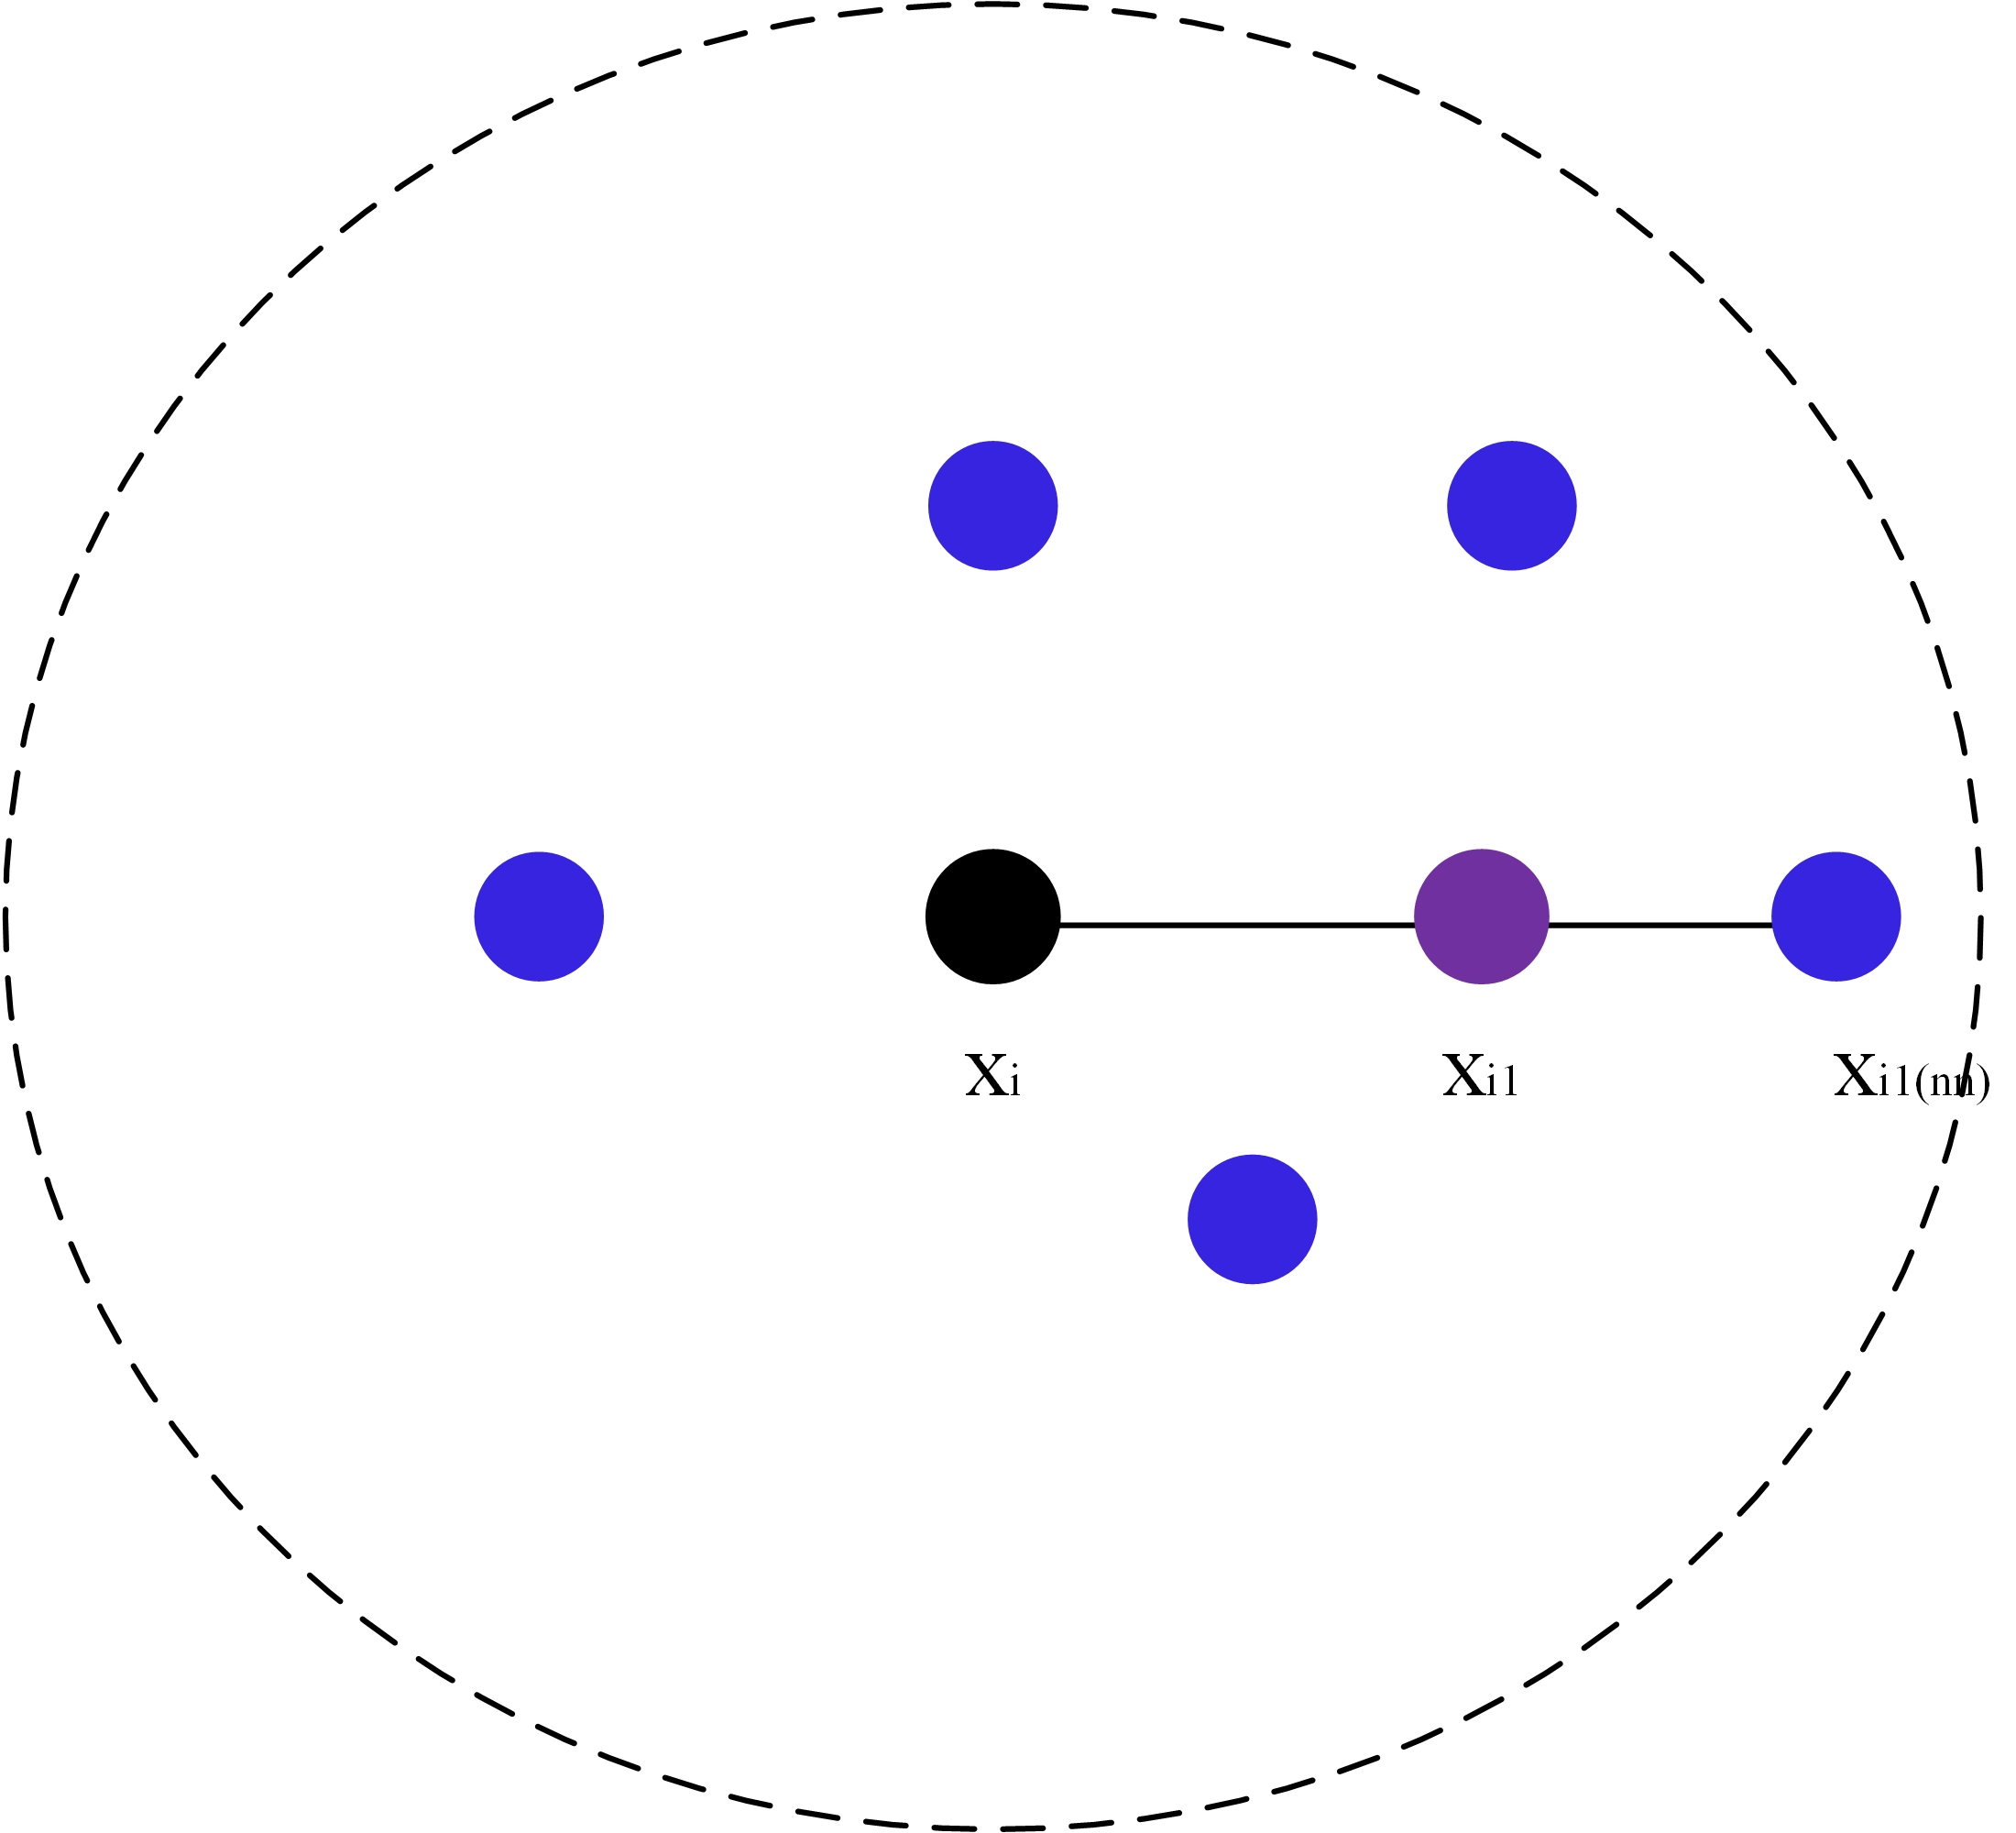
\includegraphics[width=8cm]{example/smote.jpg}
	\bicaption[SMOTE生成样本过程示意图]
	{SMOTE生成样本过程示意图}
	{Diagram of generating a sample by SMOTE.}
	\label{fig:smote}
\end{figure}

首先利用K近邻思想找到扩充样本的临近样本点,随机选取设训练集样本大小为$T$,SMOTE算法将把数据集扩充成$NT$个新样本。新样本根据式\ref{eq:smote}进行合成。
\begin{equation}
	\label{eq:smote}
	{x_{i1}} = {x_i} + {\varepsilon _1}({x_{i(nn)}} - {x_i})
\end{equation}
其中,${x_{i(nn)}}$是样本$x_i$的k近邻中任意选取的一个,$\varepsilon _1$是0到1之间的随机数,这里$x_{i1}$即为对第$i$条进行一次扩充后得到的新的样本。对于所有的T个样本进行$N$次扩充最后得到的扩充数据即为新样本集。
SMOTE算法描述如算法\ref{al:smote}所示。

\begin{algorithm}[htbp]
	\caption{SMOTE算法}% Ëã·¨±êÌâ
	\label{al:smote}
	\begin{algorithmic}[1]%Ò»ÐÐÒ»¸ö±êÐкÅ
		%\Require {The number of critic iterations per generator iteration $n_{critic}$,the batch size $m$, training iteration is $K$.}
		%\Require ~~ \\
		\Require
		数据扩充倍数$N$
		\For{$i=1$ to $T$}
		\For{$times=1$ to $N$}
		\State 对于样本$x_i$利用欧式距离找到其对应的$k$个近邻,记为${x_{i(near)}}$,$near\in\left\{ {1,...,k} \right\} $
		\State
		从$k$个近邻中随机选择一个样本${x_{i(nn)}}$,生成一个0到1之间的随机数$\varepsilon$,利用式\ref{eq:smote}生成一个新样本。
		\EndFor
		\State 对于第$i$个样本合成$N$个新样本:${x_{inew}},new \in 1,...,N$。
		\EndFor
	\end{algorithmic}
\end{algorithm}
简单进行数据的插值工作没有从模型内部学习数据的分布,可能会生成一些无法表示数据信息的无效样本。因此学习数据潜在分布的目的并没有效解决。
\section{GAN数据扩充方法}
生成式对抗网络于2014年被蒙特利尔大学的Goodfellow Ian首次提出,其在图像领域的出色表现引起了业界学者的广泛关注。利用GAN思想进行数据扩充应运而生。下面分别介绍GAN,WGAN,和VAEGAN算法。
\subsection{GAN算法}
作为Actor-Critic框架下的一员,生成式对抗网络主要有两个部分组成:生成器(Generator)和判别器(Discriminater)。生成器是生成式模型,主要学习数据的联合概率分布,图\ref{fig:GAN2}示意了GAN两个组成部分之间的关系。

\begin{figure}[htbp]
	\centering
	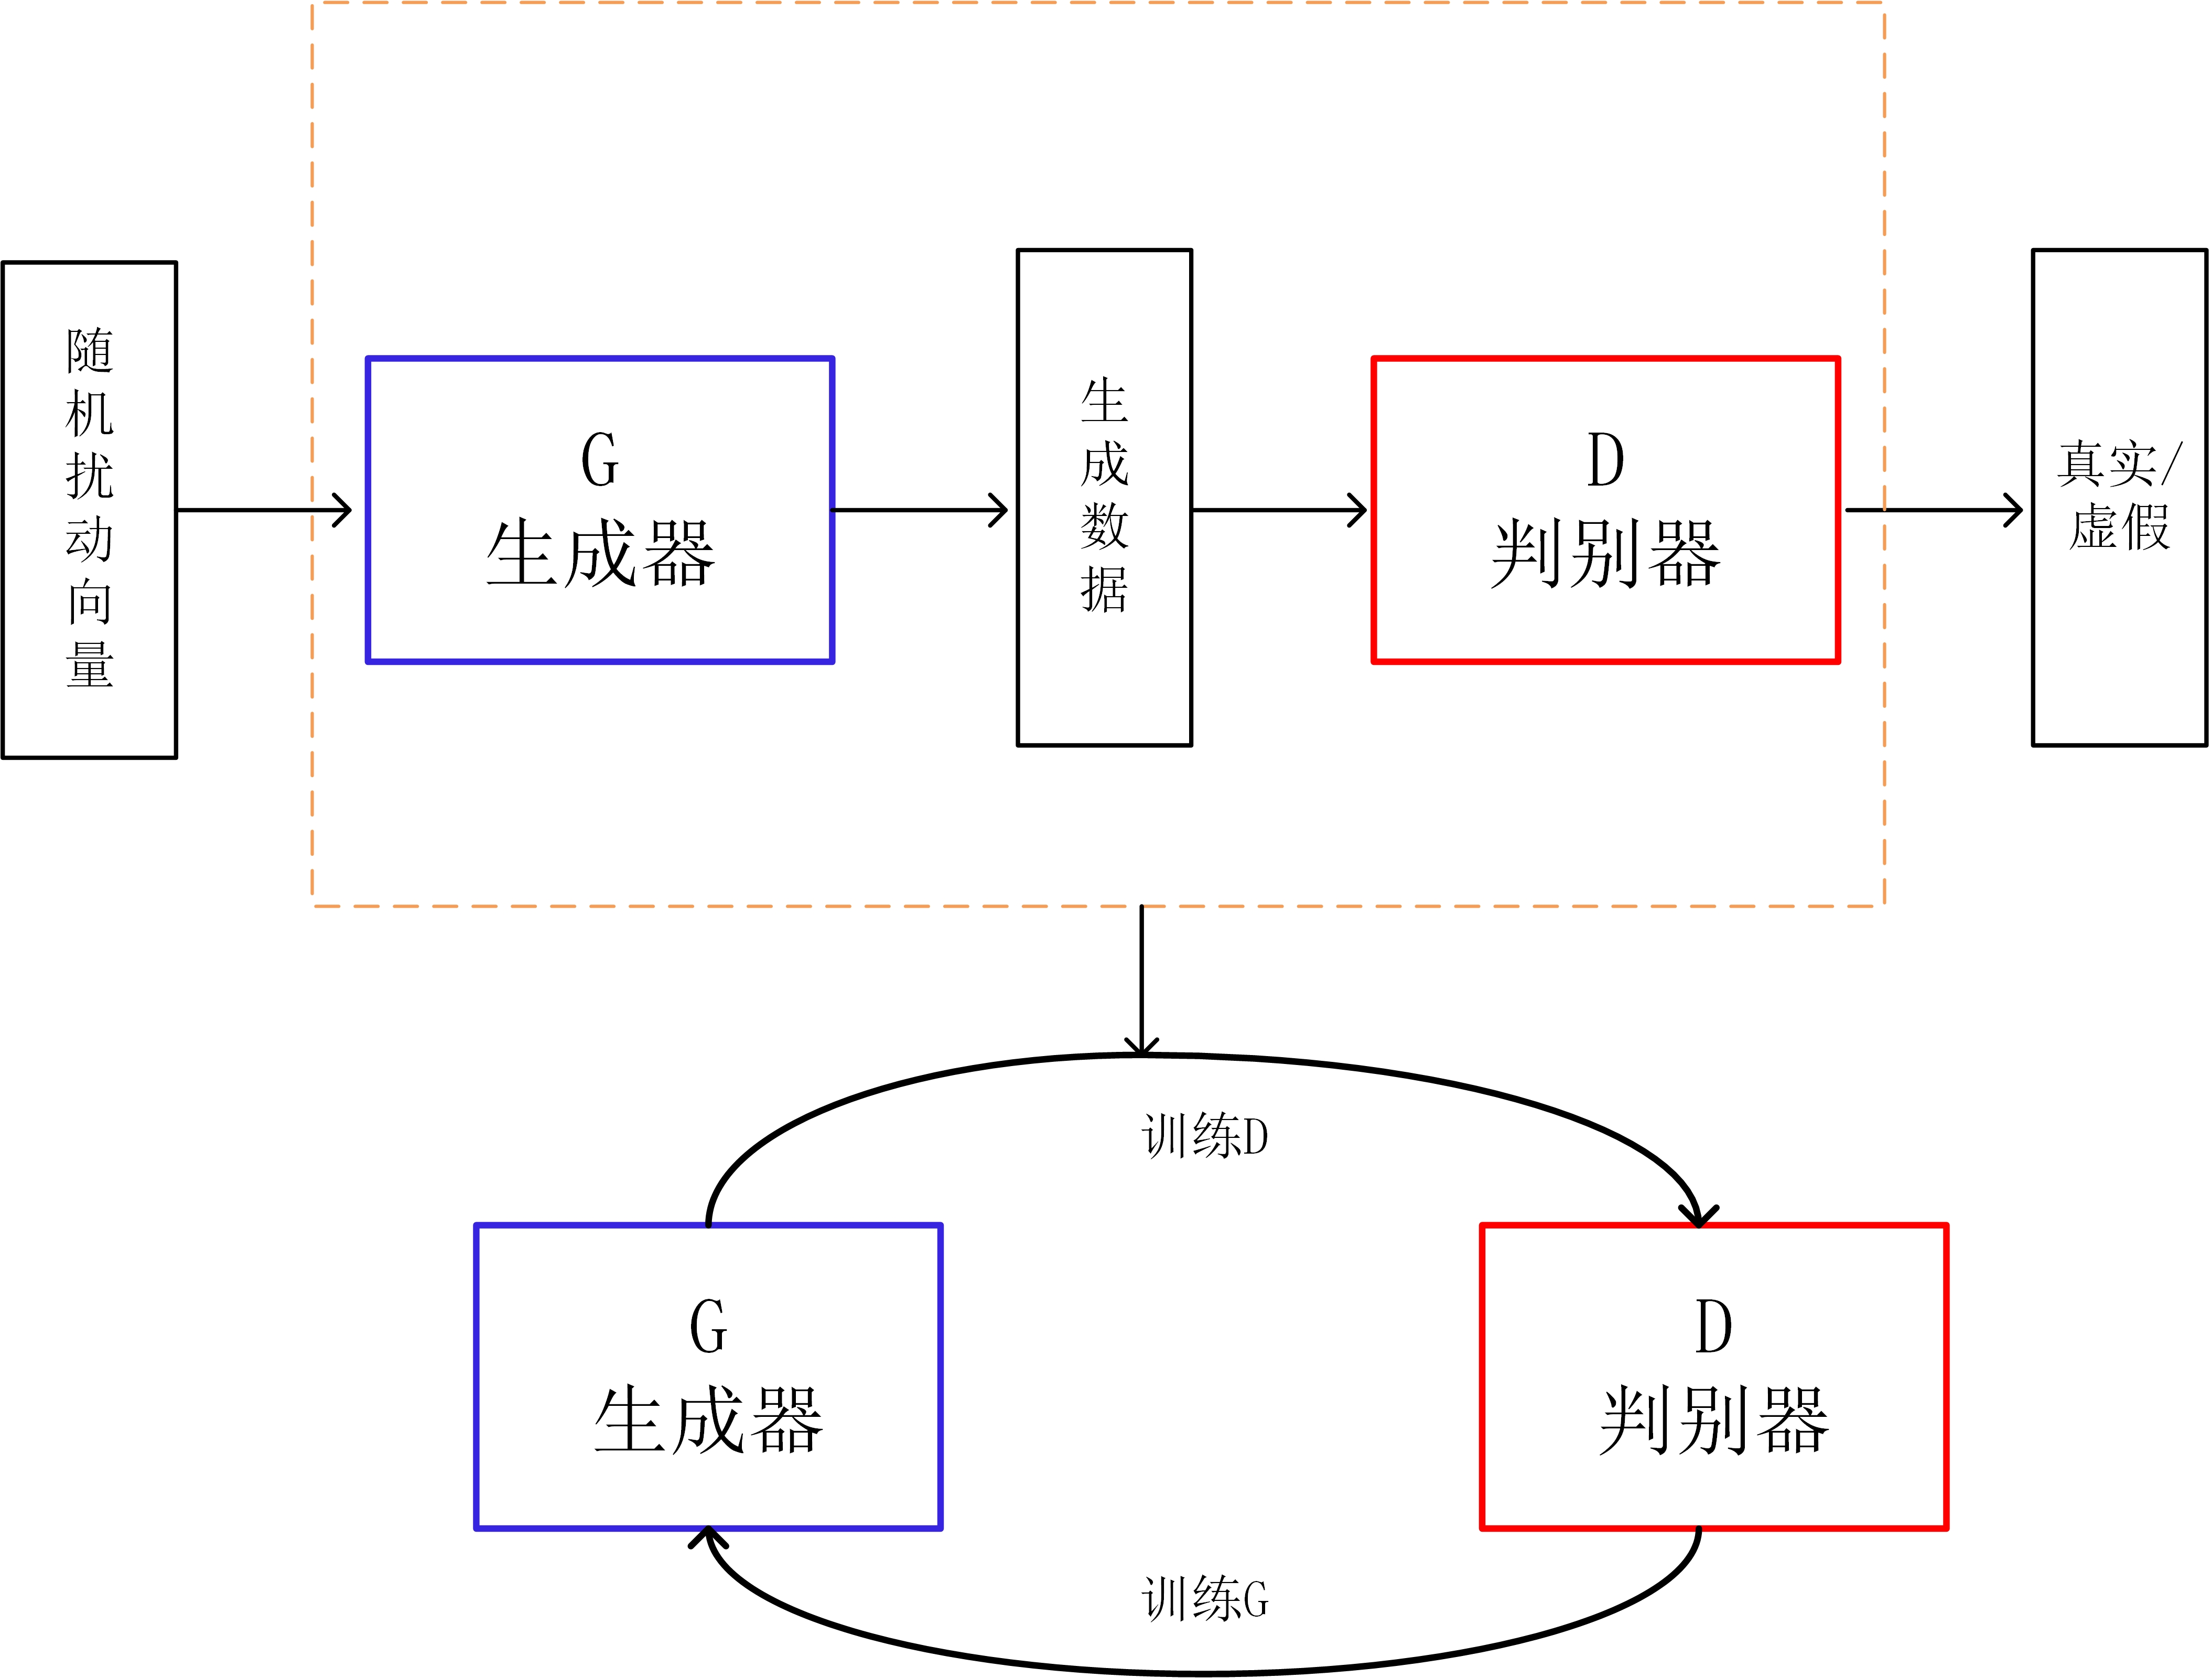
\includegraphics[width=\hsize]{example/GANframwork.jpg}
	\bicaption[GAN结构示意图]
	{GAN结构示意图}
	{Framework of GAN}
	\label{fig:GAN2}
\end{figure}
其输入的数据为任意分布的噪声,输出的数据为学习的假样本,判别器相当于一个二分类模型,其输入的数据为原始真实数据和生成器生成的假数据,输出的是输入样本属于真实样本的概率。GAN利用零和博弈模型把生成式模型和判别式模型整合在了一个框架下。对应于强化学习,GAN里面的生成器相当于智能体,生成器生成的数据就是智能体进行的动作,判别器相当于环境反馈的奖励,当生成的数据越接近真实数据,奖励值越大,生成器会向着该方向更新参数,反之当生成的数据离真实样本分布越远,奖励越小,生成器参数向反方向更新。其中,生成器和判别器可以是任何框架下的模型,通常在应用中都使用深层神经网络进行生成器和判别器的构造。

GAN作为生成式模型,求联合概率密度函数离不开极大似然估计,似然估计函数如式\ref{eq:EM}:

\begin{equation}
\label{eq:EM}
\max \limits_{\theta\in R^{d}}\frac{1}{m} \sum_{i=1}^m \log P_{\theta}(x^{(i)})
\end{equation}
在这里,$P_{\theta}$ 是密度函数的参数, $\{x^{(i)}\}^{m} _{i=1}$是从真实数据中采样得到的采样数据。
生成式对抗网络的优化目标函数可以用\ref{eq:22}函数描述。
\begin{equation}
\label{eq:22}
G^{*}=\arg \min \limits_{G} \max \limits_{D} V(G,D)
\end{equation}
这里:
\begin{equation}
\label{eq:33}
V=E_{x\sim P_{data}} [\log D(x)]+E_{x\sim P_{G}}[\log (1-D(x))]
\end{equation}
其中,$P_{data}$代表真实数据的分布,$P_{G}$ 代表生成器学习 $G$得到的假的数据的分布。 $D$ 代表判别器。当我们确定生成器和判别器都是神经网络时,用${\theta _g}$和${\theta _p}$ 分别代表生辰器和判别器的网络结构参数。定义输入的噪声数据为$ {p_z}(z)$,用${\rm{G(z,}}{\theta _g}{\rm{)}}$表示生成器对数据从噪声分布到学习数据分布的映射关系。$D(x,{\theta _d})$输出单变量代表概率值。式\ref{eq:33}整理为:
\begin{equation}
\label{eq:44}
\mathop {\min }\limits_G \mathop {\max }\limits_D v(D,G) = {E_{x \sim {p_{data}}(x)}}[\log D(x)] + {E_{z \sim {p_z}(z)}}[\log (1 - D(G(z)))]
\end{equation}
 这是一个极小极大化的损失函数,对于一个固定的$G$,对$D$求解其最优函数:
 \begin{equation}
 \label{eq:34}
 {D^*}(x) = \frac{{{p_{data}}(x)}}{{{p_{data}}(x) + {p_g}(x)}}
\end{equation}
 类似地,对于固定的$G$,求$D$的目标是最大化损失函数:
\begin{equation}\label{eq:36}
\begin{split}
v(G,D) =& \int_x {{p_{data}}(x)\log (D(x))}\mathrm{d}x + \int_z {{p_z}(z)\log (D(z))}\mathrm{d}x  \\
=&  \int_x \bigg( {{p_{data}}\log ({\rm{D}}(x)) + {p_g}(x)\log (1 - D(x))\bigg)}\mathrm{d}x 
\end{split}
\end{equation}
所以式\ref{eq:33},\ref{eq:22}可以整理为:
\begin{equation}
\label{eq:35}
\begin{split}
\mathop {\max }\limits_D v(G,D) =& {E_{x \sim {p_{data}}}}[\log {D^*}_G(x)] + {E_{x \sim {p_g}}}[\log (1 - {D^*}_G(x))] \\
=& {E_{x \sim {p_{data}}}}[\log \frac{{{p_{data}}(x)}}{{{p_{data}}(x) + {p_g}(x)}}] + {E_{x \sim {p_g}}}[\log \frac{{{p_{data}}(x)}}{{{p_{data}}(x) + {p_g}(x)}}]
\end{split}
\end{equation}
整理后得到:
\begin{equation}
\label{eq:37}
\mathop {\max }\limits_D v(G,D) =  - \log 4 + KL({p_{data}}||\frac{{{p_{data}} + {p_g}}}{2}) + KL({p_g}||\frac{{{p_{data}} + {p_g}}}{2})
\end{equation}
其中$KL$ 项表示$KL$散度\cite{joyce2011kullback},是衡量两个数据分布之间距离的函数。整理成$ JS $ 散度衡量变成:
\begin{equation}
\label{eq:38}
\mathop {\max }\limits_D v(G,D) =  - \log 4 + 2JSD({p_{data}}||{p_g})
\end{equation}

可以证明当生成器和判别器的有足够的泛化拟合能力时,对于固定的生成器,判别器都可以达到最优,然后最大化$\mathop {\max }\limits_D v(G,D) = {E_{x \sim {p_{data}}}}[\log {D^*}_G(x)] + {E_{x \sim {p_g}}}[\log (1 - {D^*}_G(x))]$ 求最优的生成器。最后$P_g$将收敛于${p_{data}}$。生成器和判别器是建立在零和博弈模型下优化目标互为相反数的网络。GAN算法描述如算法\ref{algo:GAN}所示。

\begin{algorithm}[htpb]
	\caption{GAN 算法}% Ëã·¨±êÌâ
	\label{algo:GAN}
	\begin{algorithmic}[1]%Ò»ÐÐÒ»¸ö±êÐкÅ
		%\Require {The number of critic iterations per generator iteration $n_{critic}$,the batch size $m$, training iteration is $K$.}
		%\Require ~~ \\
		\Require
		对于生成器每次更新,判别器更新的次数$n_{critic}$,批训练样本大小$m$,训练迭代次数为 $K$
		\For{$t=1$ to $K$}
		\For{$i=1$ to $n_{critic}$}
		\State 从噪声数据$Z$中采样$m$个数据:${z^{(1)},...,z^{(m)}}$
		\State
		从真实数据$X$中采样$m$个数据:${x^{(1)},...,x^{(m)}}$ 
		\State 利用随机梯度上升法更新判别器网络参数:
		\begin{equation*}
			{\nabla _{{\theta _{\rm{d}}}}}\frac{{\rm{1}}}{m}\sum\limits_{i = 1}^m {[\log D({x^{(i)}}) + \log (1 - D(G({z^{(i)}})))]} 
		\end{equation*}
		\EndFor
		\State 从噪声数据$Z$中采样$m$个数据:${z^{(1)},...,z^{(m)}}$
		\State
		从真实数据$X$中采样$m$个数据:${x^{(1)},...,x^{(m)}}$ 
		\State 利用随机梯度下降法更新生成器网络参数:
		\begin{equation*}
		{\nabla _{{\theta _g}}}\frac{{\rm{1}}}{m}\sum\limits_{i = 1}^m {\log (1 - D(G({z^{(i)}})))}
		\end{equation*}
		\EndFor
	\end{algorithmic}
\end{algorithm}

\subsection{WGAN算法}
由于原始的GAN算法存在以下三个难以解决的问题\cite{12}:
\begin{enumerate}
	\item 模式崩溃(Mode collapse),也是GAN算法最大的不足。模式崩溃指生成器更倾向于生成具有较高概率密度的数据,对于出现次数较少的数据生成器缺少对其学习表征的能力。因此导致模型生成的数据过于单一不能完整覆盖到所有样本集。
	\item 梯度消失问题,是指由于判别器学习的速度大于生成器,因此很容易区分真假数据,经过神经网络的层层传递导致梯度消失或爆炸,导致网络无法正常更新。
	\item 无法实时的评价生成数据的质量。这是由于衡量数据分布的函数是JS散度,当两组数据在空间中完全不相交时,JS散度为定值,不能直接反映出两个数据的接近程度。
\end{enumerate}
针对以上问题,WGAN\cite{arjovsky2017wasserstein}算法提出了以下两点改进:
\begin{enumerate}
\item  利用Wasserstein距离(Earth-Mover (EM) distance or Wasserstein distance )代替原来的JS散度来衡量两个数据分布的距离。
\item 为了满足判别器符合一阶利普西茨(1-Lipschtiz)条件,对两组数据连线的中点进行采样。
\end{enumerate}

Wasserstein距离的定义如下:

\begin{equation}
\label{eq37}
W(P_{data},P_{G})= \inf \limits_{\gamma \sim \prod (P_{data},P_{G})} E_{(x,y)\sim\gamma}[\mid\mid x-y\mid\mid]
\end{equation}
其中${ \prod (P_{data},P_{G})}$代表所有以 $P_{data}$ 为 $P_{G}$为边缘概率分布的联合分布$\gamma(x,y)$ 的集合。Wasserstein距离直观意义是数据从一个分布变成另一个分布所需要的最小代价,当数据分布的支撑集位于低维流形,在这里Wasserstein距离是处处连续可导的,Wasserstein距离的平滑性要优于JS散度和KL散度。根据Kantorovich-Rubinstein对偶性,式\ref{eq37}整理为:
\begin{equation}
\label{eq38}
W(P_{data},P_{G})= \frac{1}{K} \sup \limits_{\| f \| _{L} \leq K} E_{x\sim P_{data}}[f(x)]-E_{x\sim P_{G}}[f(x)]
\end{equation}
WGAN优化的损失函数为:
\begin{equation}
\label{eq39}
V= \max \limits_{D\in 1- Lipschitz} E_{x\sim P_{data}}[D(x)]-E_{x\sim P_{G}}[D(x)]
\end{equation}
improved WGAN 为了使$D$满足一阶利普西茨条件,目标函数可以用以下公式表达:
\begin{equation}
\label{eq10}
\begin{aligned}
L=&\mathop{E}_{\tilde{x} \sim P_{G}}[D( \tilde{x})]- \mathop{E}_{x \sim P_{data}}[D(x)]+ \\&\lambda \mathop{E}_{\hat{x}\sim P_{ {penalty}}} [(\| \nabla _{  \hat{x}} D(\hat{x}) \|_{2} - 1)^{2}]
\end{aligned}
\end{equation}
在这里,$\hat{x}\sim P_{ {penalty}}$被定义为从真假数据各随机采样一个数据,他们之间连线的中点所构成的数据分布,Wasserstein距离下判别器能够持续给生成器提供梯度。此外,WGAN另一个显著优势是,其值函数与生成数据分布与原始数据分布之间的差异直接相关,而GAN并非如此。
图\ref{fig:GAN1}展示了improved GAN 原论文中改进的WGAN相对于传统的DCGAN,LSGAN,WGAN 在图像生成上取得的效果对比。在这里生成器和判别器可以用全连接层,也可以用CNN。可以看出在没有经过批归一化的网络或者没有经过适当调参的网络上提升WGAN表现要好于其他三种算法。因此WGAN相对而言要容易收敛。
\begin{figure}[htbp]
	\centering
	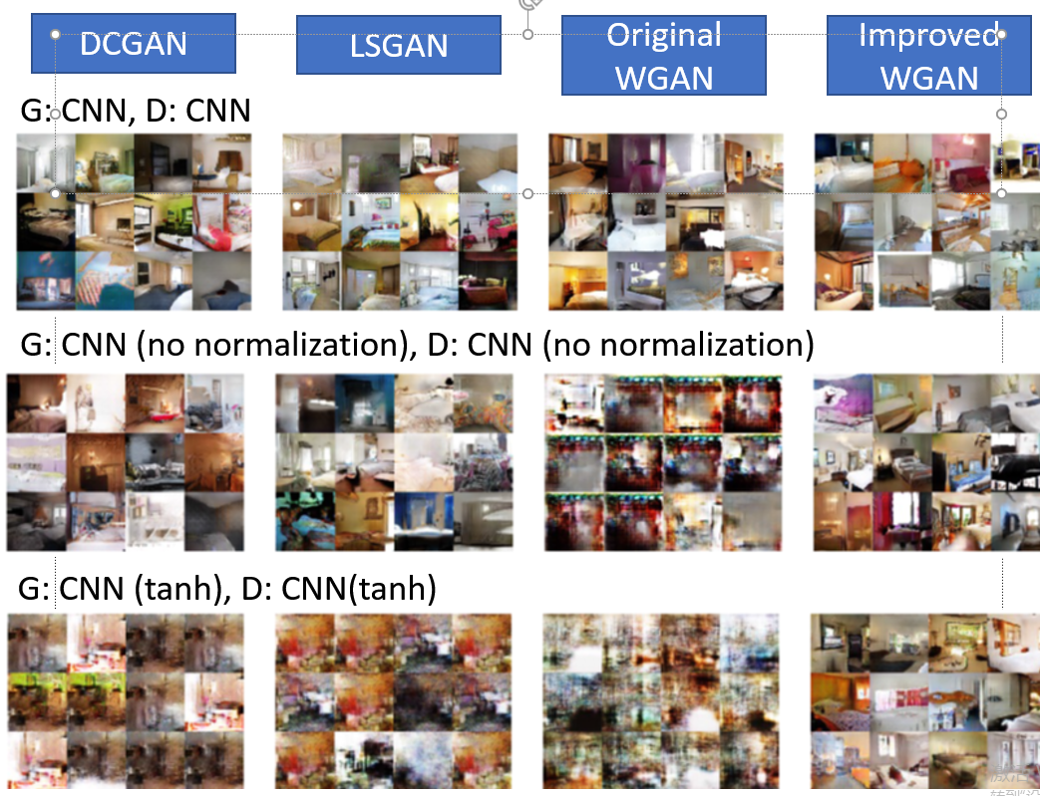
\includegraphics[width=\hsize]{example/WGAN1.jpg}
	\hspace{1cm}
	\bicaption[不同GAN在图像上的效果]
	{不同GAN在图像上的效果}
	{The effect on the image of diffent GANs.}
	\label{fig:GAN1}
\end{figure}

\subsection{VAEGAN算法}
VAEGAN将在GAN鉴别器中学习到的特征表示作为VAE的基础。与原始的VAE相比,VAEGAN将元素误差替换为特征误差,以更好地捕获数据分布,同时提供不变量\cite{7}。VAE的理论是概率变分界\cite{16},即:

\begin{equation}
p(x)\geq E_{q(x\mid z)}[log p (x\mid z)]- KL(q(z\mid x)\parallel P (z))
\end{equation}

然而,由于VAE的结构,VAEGAN不得不遵循这样的假设:潜在变量可以通过分解高斯分布很好地拟合。在上述约束条件下,编码器将实际样本转化为隐向量空间,使生成的潜在向量大致服从正态分布。VAEGAN使用GAN的鉴别器作为一种学习相似性度量,但没有利用GAN强大的生成能力。在数据的重构和修复上有很好的效果,但是在数据增强表现一般。VAE是基于隐向量向量可以近似为高斯分布的假设,使得GAN也必须满足这种假设,强约束的加入限制了GAN的生成能力。

虽然WGAN解决了梯度消失的问题,并提供了生成样本的直接评价准则,但是没有对象能够保证遍历所有模式的样本。模式崩溃仍然是一个主要问题。生成器的输入是高斯噪声,其随机性导致训练过程不稳定,收敛缓慢\cite{17}等问题,这种现象在训练初期尤为明显。

\section{改进的有监督信号的WGAN算法}
如前面内容提到的,GAN主要应用于图像视频领域,对于非图像类数据还没有良好的应用效果。在这一节,将详细介绍一种有监督信号的WGAN算法,本章提出的算法主要结合了自动编码机(Auto-Encoder,AE)模型学习隐向量的表征能力和WGAN提供持续梯度的优势。通过自动编码机模型引入监督信号,改进了生成样本覆盖不均不能有效监测训练过程的缺陷。
\subsection{引入监督信息}
监督学习模型因为其优化的目标函数具有规则的几何形状,所以可以有效解决模型梯度消失的问题\cite{11}。真实的样本可以通过输入隐式空间向量来重建一个性能良好的模型,这样就给生成模型提供了有监督的信号。GAN中的生成器可以作为解码器把经过自动编码机编码后的隐向量进行解码操作,把压缩后的特征还原到原始特征空间$X$。在这种有监督的训练过程中,隐向量可以看作是低维空间$Z$中固定的先验分布。因此,先验知识由AE获得,这种方法在机器学习领域的编码工作中得到了广泛的应用。与VAE相比,AE没有额外的隐向量分布的限制。监督信号的优化目标可以描述为:  $ G(E(X))\rightarrow X $。最优的生成器可以最小化$ G(E(X))$和$X$之间的差异。在随机噪声数据的输入中加入规则信息,避免了大量的盲目尝试过程。能够加快模型的收敛速度,提升模型的学习能力
\subsection{改进的WGAN算法描述}
改进的WGAN的具体实现过程为,除了高斯噪声,隐式特征向量并行的作为输入数据传给生成器,作为数据生成的额外附加信息,隐向量携带着数据本身的一些信息。将AE与WGAN相结合,可以在编码器中使用学习到的特征表示作为WGAN生成目标的基础。改进算法的框架如图~\ref{fig2}所示。

\begin{figure}[htbp]
	\centering
	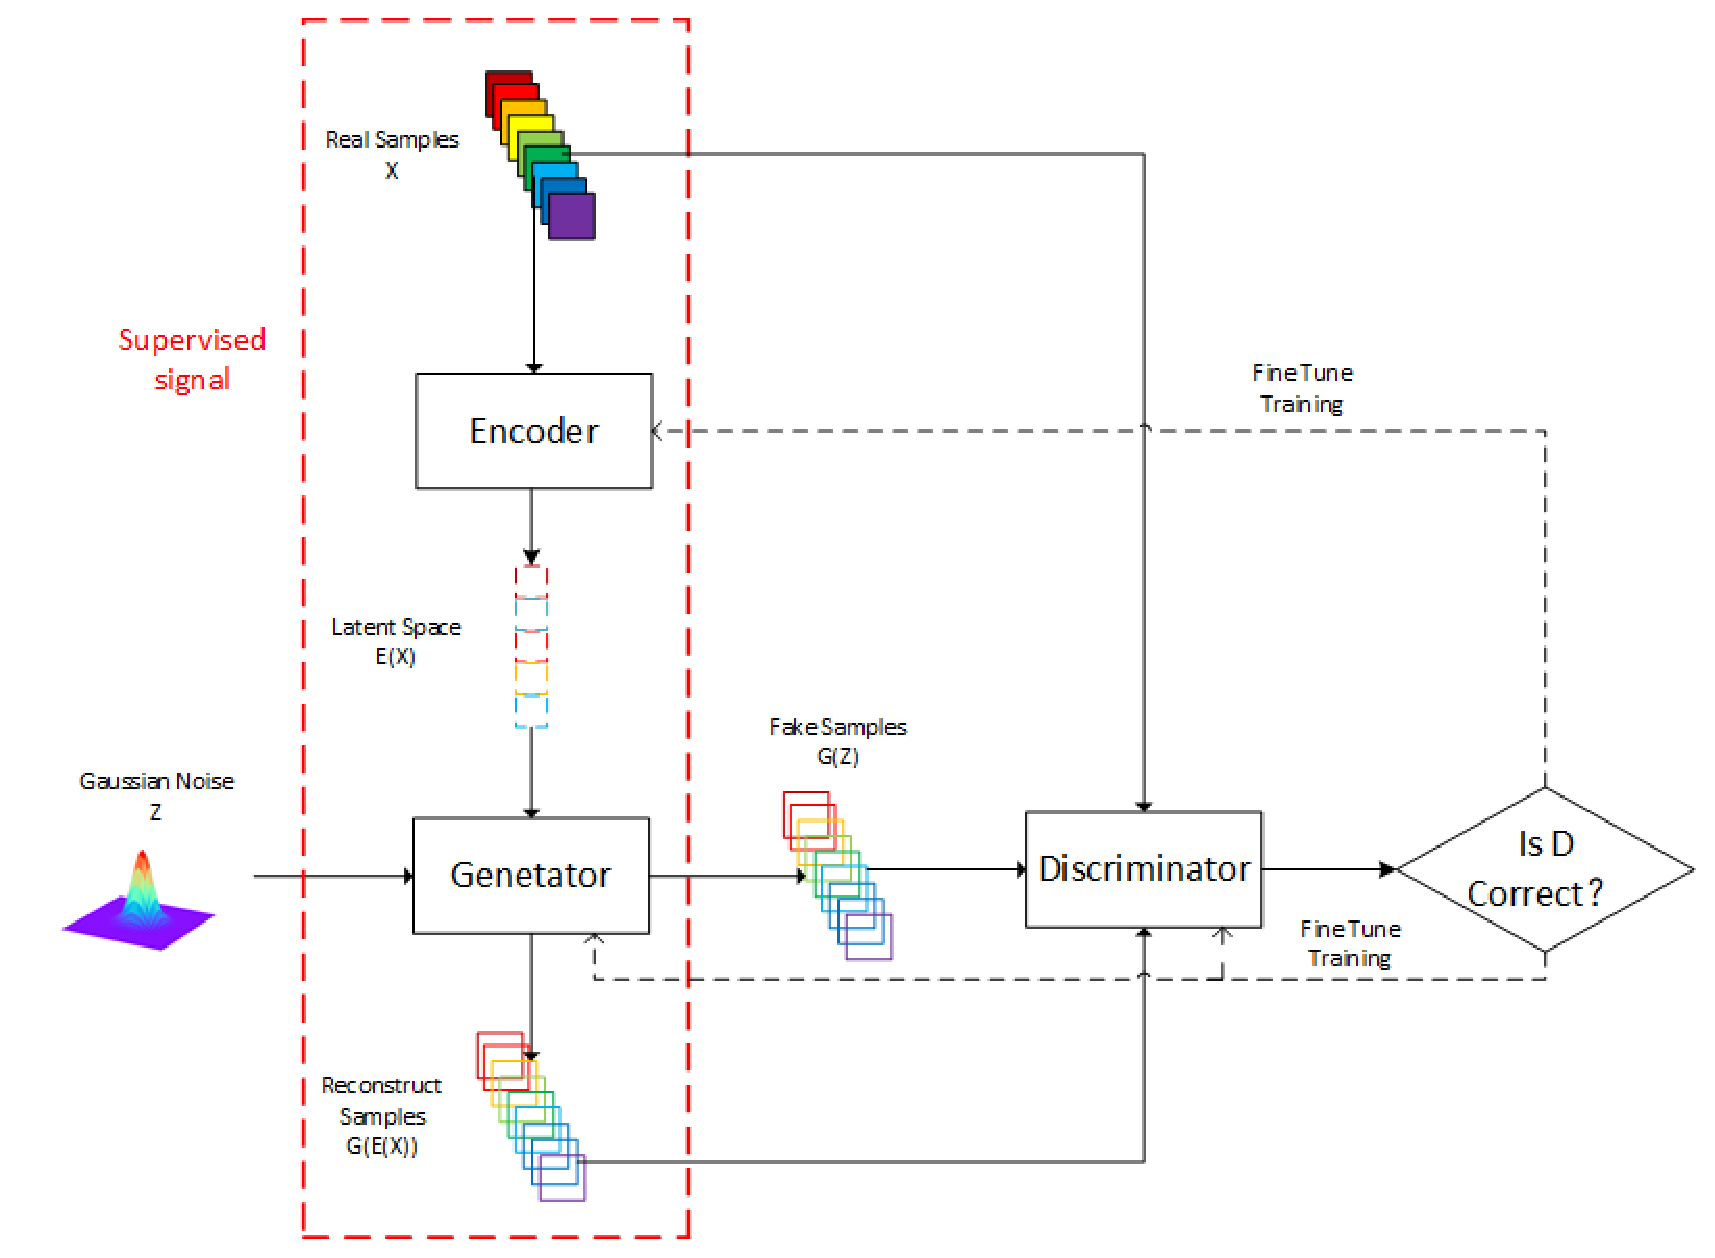
\includegraphics[width=\hsize]{example/2.eps}
	\bicaption[带监督信号的WGAN流程图]
	{带监督信号的WGAN流程图}
	{Flowchart of WGAN with Supervised Signal.}
	\label{fig2}
\end{figure}

图~\ref{fig2}中的所有样本都是数值类数据集。可以看到除噪声数据外,还将自动编码机获得的隐向量数据表示形式输入到生成器中。生成器将隐向量转换为重构样本,优化的目标是期望重构样本尽可能接近真实样本。判别器通过最大限度地提高真样本和假样本的差异,从假样本、重构样本和真样本中获取信息。同时,生成器的目标是产生判别器无法区分的伪样本。判别器和生成器的训练过程是对抗性的。因为带监督信息的编码机能够遍历所有的原始样本,在原始数据中所有的分布都可以被模型学习到。有监督信号有助于学习到的概率密度函数能够均匀的分布在所有有原始样本的空间,从而为模态崩溃提供了有效的解决方案。元素方向误差是在原有特征方向误差的基础上提高整体结构稳定性的一种方法。

在这里,编码器用于获取数据潜在的特征数据,通过最小化像素级别的误差 $ L ^ { 2 } $距离来提供更多信息:

\begin{equation}
\label{eq11}
T_{encoder} = D_{reconstruction}=\parallel X-G(E(X))\parallel^{2}
\end{equation}

这么做的好处是生成器可以将噪声样本$Z$和潜在样本$E(X)$分别转化为伪样本和重构样本,并从判别器那里获得较高的置信度。和原来的WGAN类似,这里我们仍旧使用Wasserstein距离作为统计标准来衡量两个数据分布的接近程度。这样经过引入了监督信号,新的算法优化目标函数变为:
\begin{equation}
\label{eq:12}
T_{G} = -D(G(Z))-D(G(E(X)))+\parallel X-G(E(X))\parallel^{2}
\end{equation}

这里面$Z$ 是从简单的噪声分布中采样得到的数据,噪声的分布可以是均匀分布或者是高斯分布。对于判别器,$X$ 是真实的数据,$G(Z)$ 和 $G(E(X))$都是假样本。这个过程的优化目标函数可以描述为:

\begin{equation}
\label{eq12}
T_{D} = D(X)-D(G(E(X)))-D(G(Z))
\end{equation}

有监督信号的WGAN算法的流程如算法\ref{al:improved WGAN}所示。

\begin{algorithm}[htpb]
	\caption{有监督信号的WGAN}% Ëã·¨±êÌâ
	\label{al:improved WGAN}
	\begin{algorithmic}[1]%Ò»ÐÐÒ»¸ö±êÐкÅ
		\Require ~~ \\
		对于生成器每次更新,判别器更新的次数$n_{critic}$,批训练样本大小$m$,训练迭代次数为 $K$.
		\For{$t=1$ to $K$}
		\For{$i=1$ to $n_{critic}$}
		\State 从噪声数据$Z$中采样$m$个数据:${z^{(1)},...,z^{(m)}}$
		\State 从真实数据$X$中采样$m$个数据:${x^{(1)},...,x^{(m)}}$ 
		\State 利用随机梯度上升法更新判别器网络参数:
		\begin{equation*}
		\nabla_{\theta_{d}}\frac{1}{m}\sum_{i=1}^m[D(x^{(i)})-\lambda {\rm{D(G(E(x^{(i)})))}}-D(G(z^{(i)}))]  
		\end{equation*}
		\EndFor
		\State 从噪声数据$Z$中采样$m$个数据:${z^{(1)},...,z^{(m)}}$
		\State 从真实数据$X$中采样$m$个数据:${x^{(1)},...,x^{(m)}}$
		\State 利用随机梯度下降法更新生成器网络参数:
		\begin{equation*}
		\nabla_{\theta_{d}}\frac{1}{m}\sum_{i=1}^m[-D(G(z^{(i)}))-\lambda {\rm{D(G(E(x^{(i)}))}}+\parallel x^{(i)}-G(E(x^{(i)})\parallel^{2}]
		\end{equation*}
		\State 利用随机梯度下降法更新自动编码器网络参数:
		\begin{equation*}
		\nabla_{\theta_{d}}\frac{1}{m}\sum_{i=1}^m[\parallel x^{(i)}-G(E(x^{(i)})\parallel^{2}]
		\end{equation*}
		\EndFor
	\end{algorithmic}
\end{algorithm}
\section{模型性能分析}
在本节将对比改进模型和其他GAN网络在高斯分布下表现以及传统数据合成方案和GAN网络在标准数据集下的表现进行模型有效性分析。
\subsection{不同GAN网络算法结果对比分析}
由于数据的分布很难直观的观察到,为了可视化数据,首先生成一维概率密度分布已知的数据,从中采样得到相应的真实样本数据,把这些真实样本数据作为GAN网络的输入数据,然后绘制输出学习到的数据分布。观察生成数据和原始真实数据的吻合程度。

首先假设原始数据分布为两个高斯分布的叠加,第一个高斯分布为$\mu=4,\sigma=0.5$,第二个高斯分布为$\mu=0,\sigma=0.3$。原始数据分布形式如图\ref{figyuanshi}。
\begin{figure}[htbp]
	\centering
	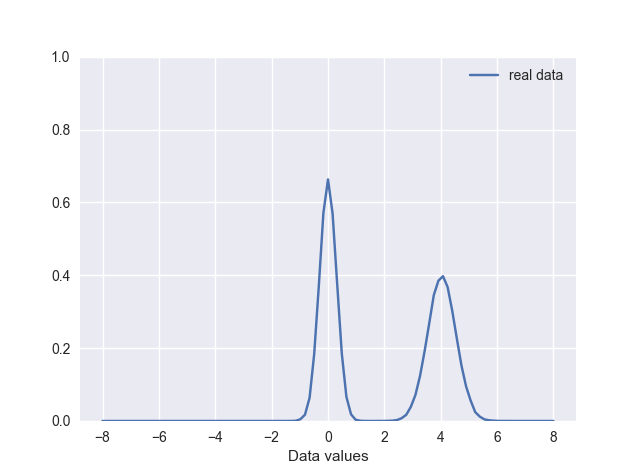
\includegraphics[width=\hsize]{example/yuanshi.png}
	\bicaption[原始高斯分布]
	{原始高斯分布}
	{Flowchart of WGAN with Supervised Signal}
	\label{figyuanshi}
\end{figure}

对比WGAN,VAEGAN和改进的GAN算法,使用相同的网络结构,扩充数据量都为10000条,绘制扩充后的数据和原始数据的概率密度对比图如图\ref{fig:shiyan}。


\begin{figure}[htpb]
	\centering
	\subcaptionbox{WGAN概率密度图\label{fig:shiyan:a}}
	{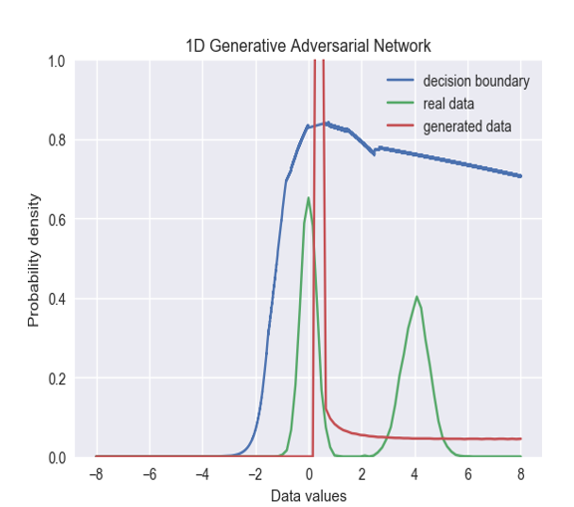
\includegraphics[width=0.45\hsize,height=0.43\hsize]{example/tu1.png}}
	\hspace{0.5em}
	\subcaptionbox{WGAN损失函数图\label{fig:shiyan:b}}
	{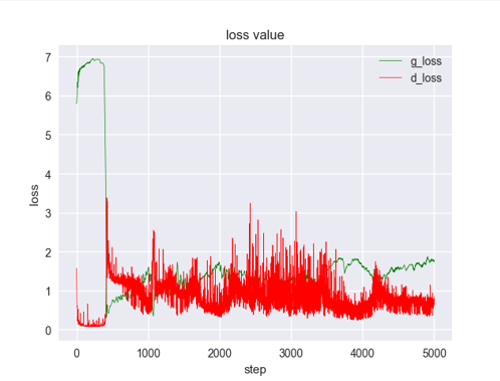
\includegraphics[width=0.45\hsize,height=0.43\hsize]{example/loss1.png}}
	\newline
	\centering
	\subcaptionbox{VAEGAN概率密度图\label{fig:shiyan:c}}
	{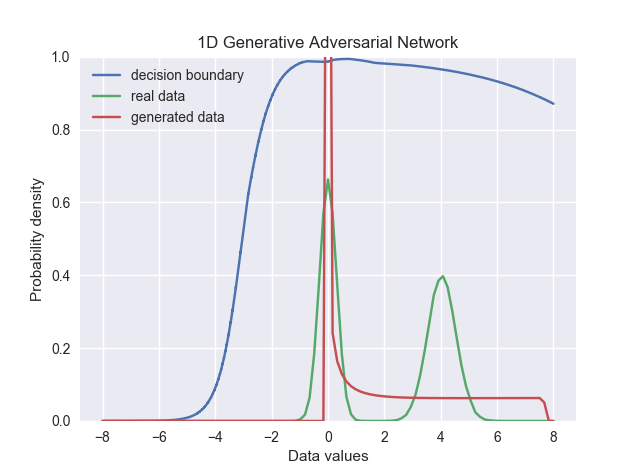
\includegraphics[width=0.45\hsize,height=0.43\hsize]{example/tu2.png}}
	\hspace{0.5em}
	\subcaptionbox{VAEGAN损失函数图\label{fig:shiyam:d}}
	{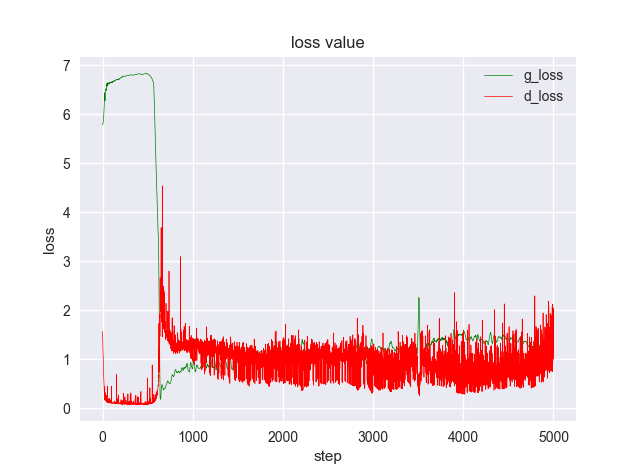
\includegraphics[width=0.45\hsize,height=0.43\hsize]{example/loss2.png}}
	\newline
	\centering
	\subcaptionbox{改进WGAN概率密度图\label{fig:shiyan:e}}
	{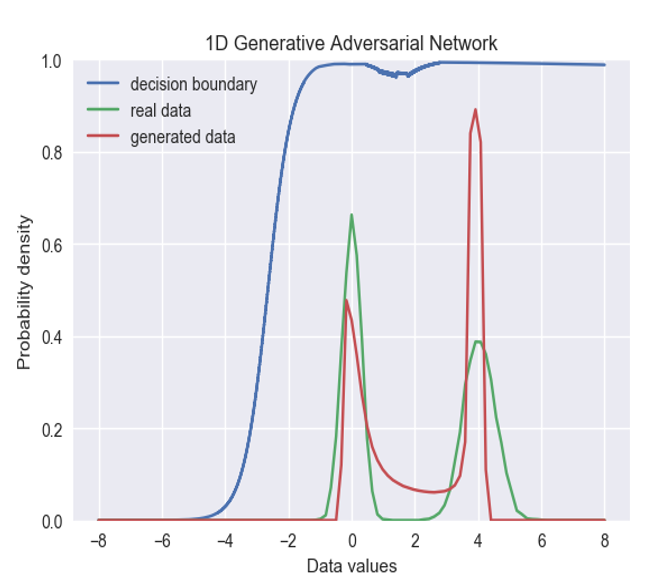
\includegraphics[width=0.45\hsize,height=0.43\hsize]{example/tu3.png}}
	\hspace{0.5em}
	\subcaptionbox{改进WGAN损失函数图\label{fig:shiyam:f}}
	{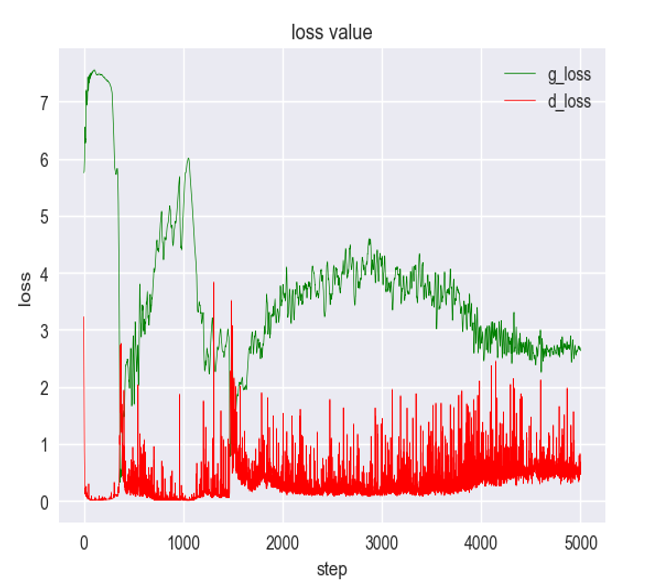
\includegraphics[width=0.45\hsize,height=0.43\hsize]{example/loss3.png}}
	\bicaption
	{不同GAN算法概率密度对比.}
	{Comparison of probability density of different GAN algorithms.}
	\label{fig:shiyan}
\end{figure}



可以看出,对于GAN算法,生成的数据只能学习到单高斯峰,而且生成的数据并不能准确描述$\mu=0,\sigma=0.3$的分布。判别器判别曲线还可能够判别出真假数据。从损失函数曲线上分析,两个网络始终没有达到相对稳定的状态。对于WGAN算法,仍然不能很好描述所有数据分布,但是由于引入了Wasserstein距离,损失函数曲线相比于GAN更加稳定,生成数据能相对准确的描述其中一个高斯分布,对于改进的WGAN算法,生成器已经能学到两个高斯分布,并且效果比前两种算法有所改善。对于损失函数生成器的损失函数大体呈下降趋势。通过对一维数据进行可视化,可以看出改进的算法在一定程度上改善了学习数据分布不全面,损失函数下降困难的问题。
\subsection{模型在标准集下的表现}
本节将结合标准数据集中联合循环发电厂(Combined Cycle Power Plant, CCPP)数据集讨论不同算法下回归数据的结果。该数据集包含了一个联合循环电厂在6年(2006-2011)的全负荷运行中收集到的9568个数据点。特征包括小时平均环境变量温度(T)、环境压力(AP)、相对湿度(RH)和排气真空(V),用于预测工厂的净小时电能输出(EP)。
数据集的描述如表\ref{tabccpp}。
\begin{table}[htpb]
	\centering
	\bicaption[CCPP数据集描述]
	{CCPP数据集描述}
	{Description of CCPP dataset.}
	\label{tabccpp}
	\begin{tabular}{llll} \toprule
		属性名   & 描述 & 数据类型&数据范围  \\  \midrule
		Temperature&温度&浮点型(连续性)&$1.81^\circ C$, $37.11^\circ C$\\
		Ambient Pressure&环境压力&浮点型(连续性)&992.89, 1033.30 milibar\\
		Relative Humidity&相对湿度&浮点型(连续性)& 25.56$\%$, 100.16$\%$ \\
		Exhaust Vacuum&排气真空度&浮点型(连续性)&25.36, 81.56 cm Hg\\
		Hourly electrical energy output&每小时电能输出&浮点型(连续性)&420.26, 495.76 MW\\ \bottomrule
	\end{tabular}
\end{table}

原始数据量为9568个,用改进的WGAN算法扩充100000个,加入原始数据中观察数据扩充效果。设定生成数据量的大小都为选用的衡量指标是均方误差,通过设置不同$lambda$参数,平衡损失函数中数据生成和数据解码之间的关系。

为了评价新算法生成的样本质量,把所有数据归一化后,采用SVR模型进行回归,这里SVR使用径向基核函数。更多的拟合先验分布的伪样本可以改善回归结果。均值平方误差(Mean squared error, MSE)是一种反映SVR回归准确率的评价标准,用于间接检验数据增强实验的有效性。MSE的定义可以用公式\ref{eq14}表示:

\begin{equation}
\label{eq14}
MSE=\frac{\sum \limits_{i=1}^m (y^{i}-\bar{y})^{2}}{m}
\end{equation}

在这里 $y^{i}$ 是SVR预测的标签值,$\bar{y}$ 是原始数据的真实标签,测试数据集中有$m$样本,MSE值越小,误差越小,得到的生成样本越好。

图\ref{figCCPP}为当生成样本数量都为10000条时,CCPP数据集在不同GAN模型下随着迭代进行回归的结果。
\begin{figure}[htbp]
	\centering
	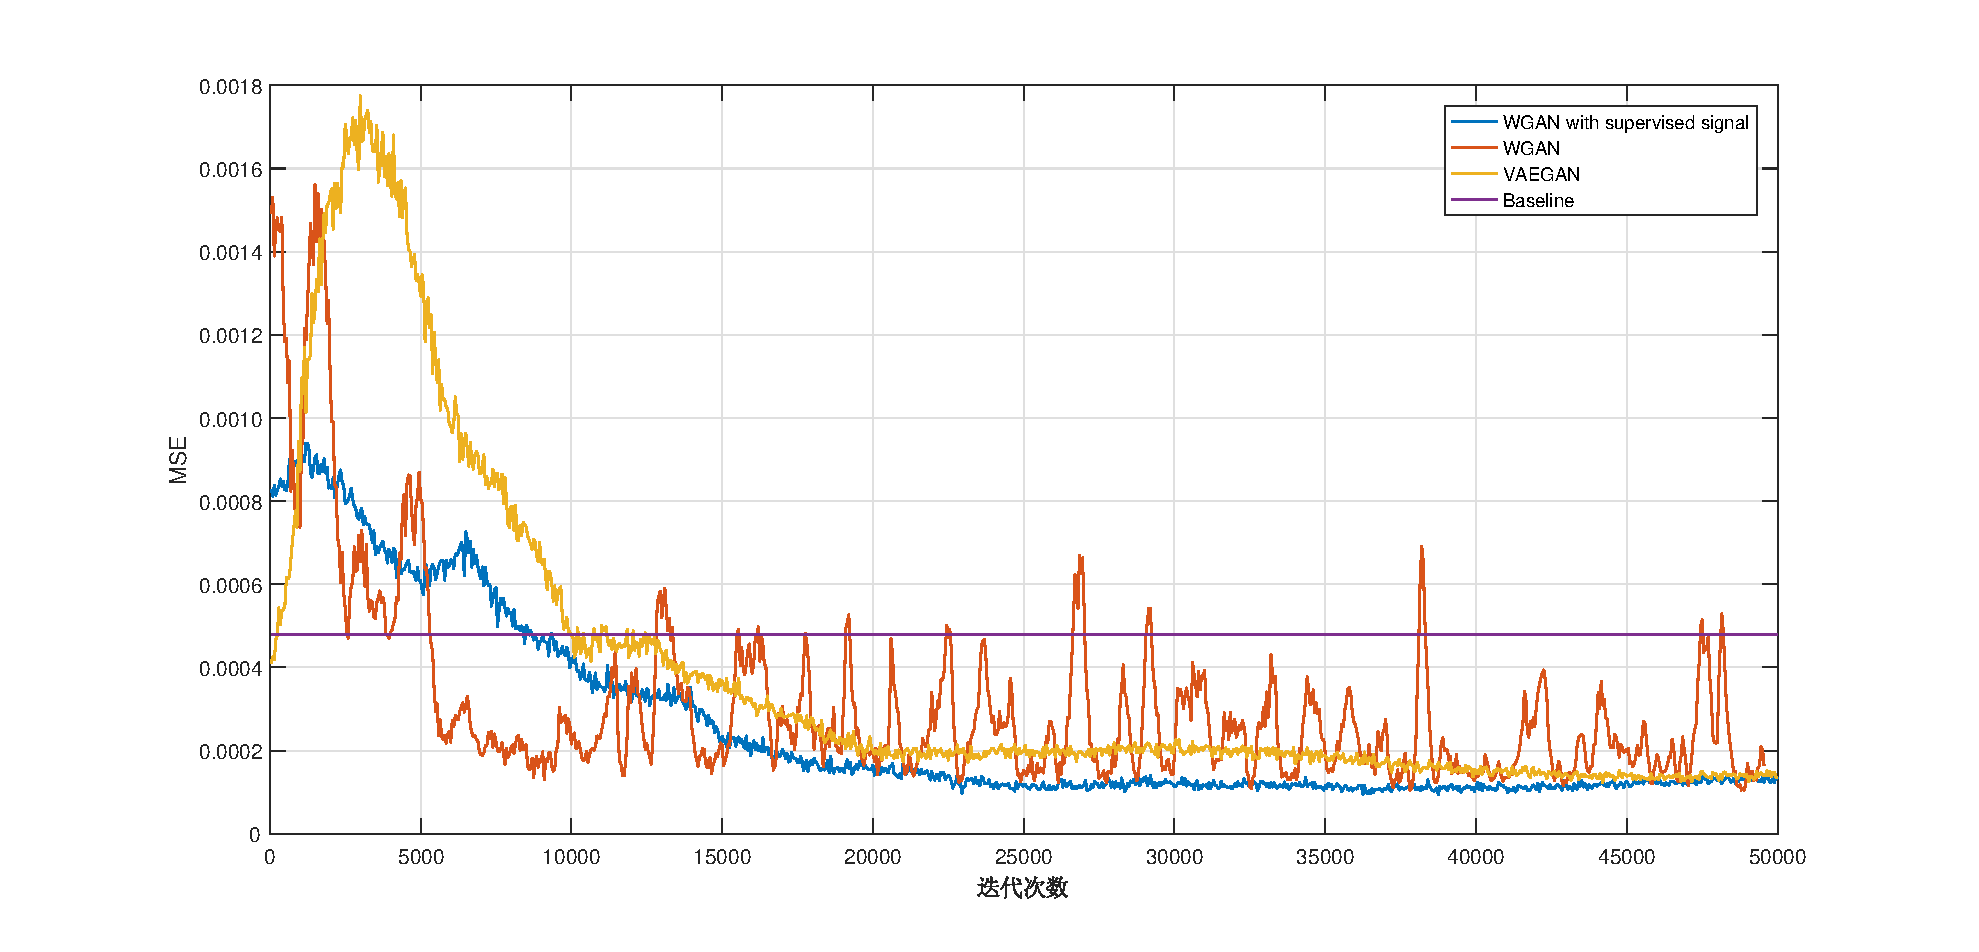
\includegraphics[width=\hsize]{example/WGANCCPP.eps}
	\bicaption[CCPP数据实验结果]
	{CCPP数据实验结果}
	{Results of CCPP dataset.}
	\label{figCCPP}
\end{figure}

对于WGAN算法回归效果在前期并不理想,后期也存在的抖动问题。分析原因是模型的难收敛性造成的,VARGAN算法在前期MSE值比较高,因为前期模型并没有得到有效的生成数据,给整个数据分布带来了大量的噪声,导致前期的MSE值要高于没有使用数据增强得到的回归MSE。在训练后期迭代次数到达12000时,MSE开始低于基准值,最后缓慢下降至一个稳定的值,改进的加入监督信号的WGAN算法在前期由于加入了自编码器的限制,模型收敛相对较快,在迭代次数大约8000次时MSE已经小于基准值。最后整体回归的表现也好好于其他模型。可以看出在迭代次数80000次后,曲线呈上升趋势,分析这是由于深度学习网络过拟合造成的,解决方案是通过监控损失函数曲线,当发现loss呈上升趋势进行早停处理。

最后所有的GAN网络取相同的迭代次数4000次,和Bootstrap算法,SMOTE算法,以及没有做数据扩充前的数据进行对比,数据扩充的数量均为原来数据的5倍,分别在标准集CCPP,CH,Servo下进行实验,得到的回归MSE值如表\ref{tabMSE}所示。同时绘制对比曲线图如图\ref{tabMSE}


\begin{table}[htpb]
	\centering
	\bicaption[标准数据集下不同模型生成数据进行回归RMSE]
	{标准数据集下不同模型生成数据进行回归RMSE.}
	{Data generated by different models were used for regression MSE.}
	\label{tabMSE}
	\begin{tabular}{lllllll} \toprule
		数据集 & 无数据扩充 & 随机加权算法&SMOTE&WGAN&VAEGAN&有监督信号的WGAN \\  \midrule
		CCPP&0.02&0.019&0.0178&0.01589&0.0147&0.0079\\
		CH&0.079&0.0788&0.06578&0.0588&0.047&0.04\\
		Servo&0.1587&0.158&0.1402&0.1388&0.1375&0.1319\\
		 \bottomrule
	\end{tabular}
\end{table}



\begin{figure}[htpb]
	\centering
	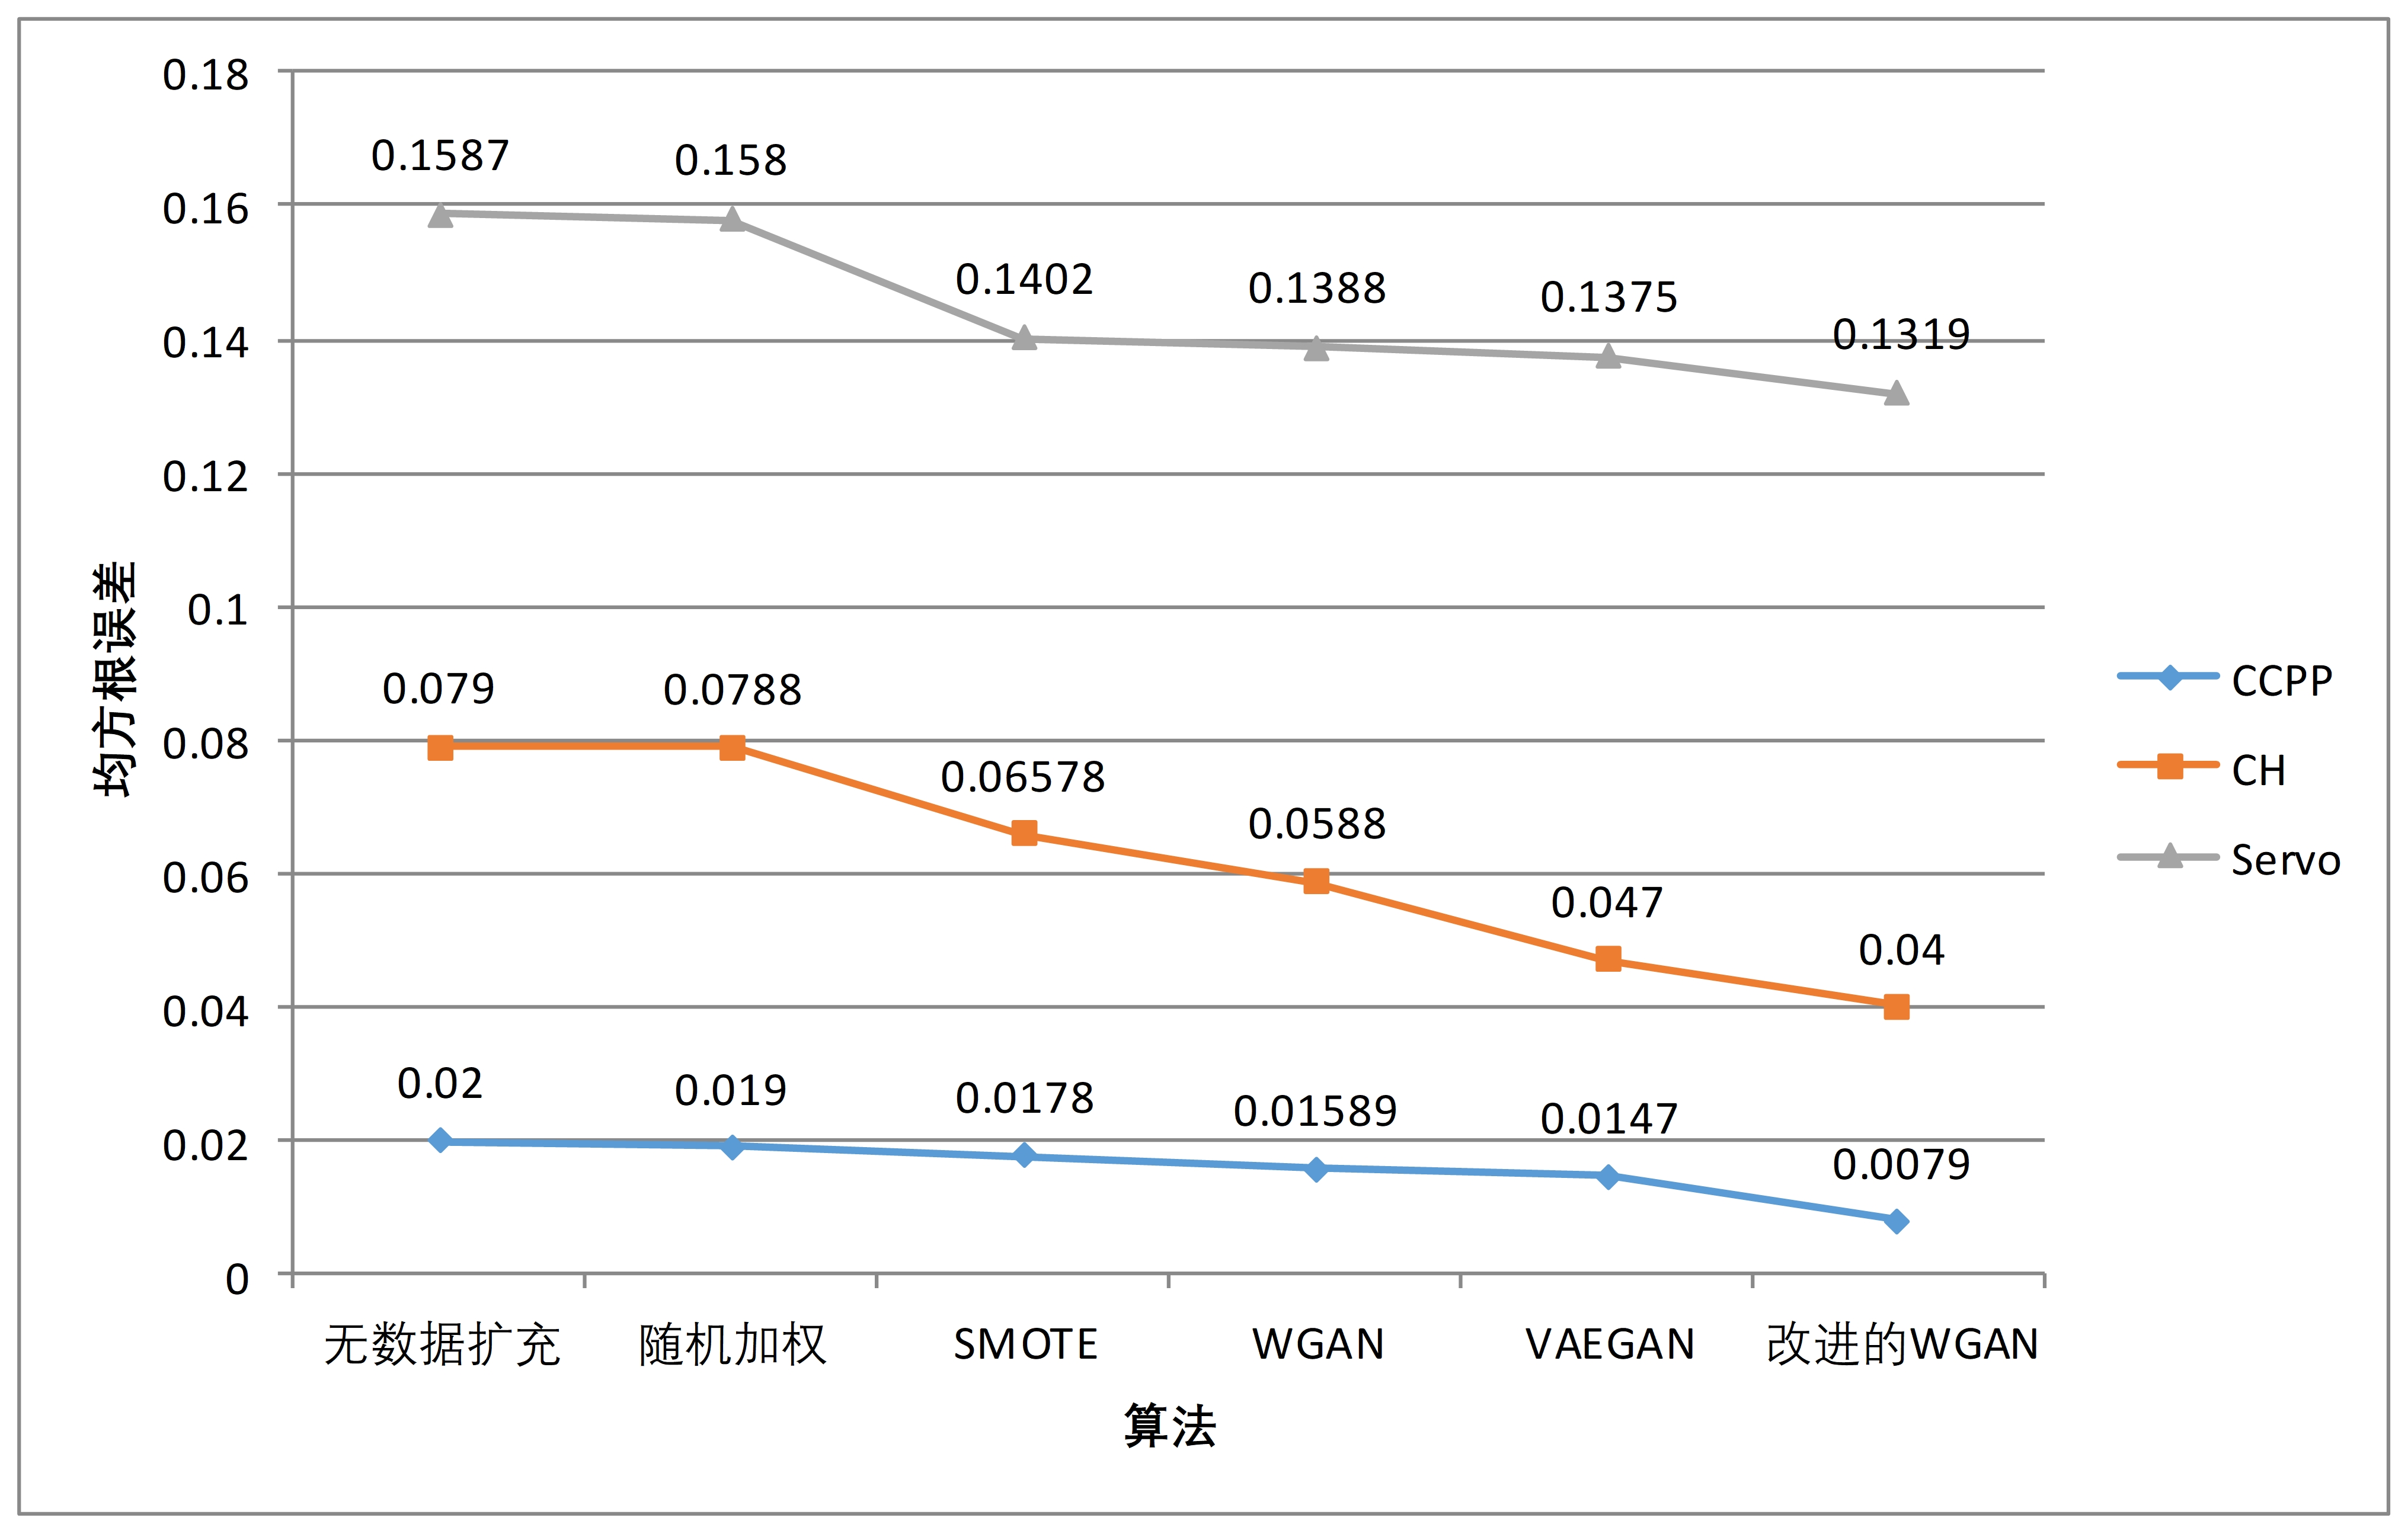
\includegraphics[width=\hsize]{example/shujujisuanfaduibi.jpg}
	\bicaption[标准数据集下不同模型生成数据进行回归RMSE曲线图]
	{标准数据集下不同模型生成数据进行回归RMSE曲线图}
	{RMSE of different methods.}
	\label{fig:MSE}
\end{figure}

可以看出,随机加权法由于没有考虑数据之间的距离随机产生数据,对回归效果提升不大,SMOTE算法利用数据插值方法一定程度上扩充了数据,但是对最后结果的提升有限,引入GAN算法的WGAN,VAEGAN相比传统算法结果会有一定提升,经过在三组标准数据集下验证,本章提出的算法无论在数据扩充效果上还是模型收敛速度上,相对于传统经典扩充算法以及其他GAN算法均有所改善。


\section{实验结果及分析}
本节将给出实际的仿真结果和相应的结论。现有的GAN训练实验大多基于图像数据或视频数据。本文将改进后的新算法应用于数值数据的扩展。

\subsection{电子设备参数实验}

本节数据集来自洛阳电子对抗基地。特征值的个数为10,输出响应变量为二维。另外,数据样本有72个,其中选择60个数据样本进行训练,选择12个样本进行测试。将改进算法应用于电子设备参数,验证了算法的稳定性。为了进行对照实验,也使用了VAEGAN和WGAN。对于编码器、解码器、生成器和判别器,所有对比模型都具有相同的架构。模型使用RMSProp优化算法进行训练,学习率为0.0003,$minibatch$大小为24。表\ref{tab3}中列出了网络架构。

\begin{table}[htpb]
	\centering
	\bicaption[有监督信号WGAN网络结构参数]
	{有监督信号WGAN网络结构参数}
	{Network structure parameters of improved algorithm.}
	\label{tab3}
	\begin{tabular}{lll} \toprule
		编码器   & 生成器 & 判别器  \\  \midrule
		12 fully-connected, ReLU &12 fully-connected, ReLU&12 fully-connected, ReLU\\
		24 fully-connected, ReLU&24 fully-connected, ReLU&24 fully-connected, ReLU\\
		24 fully-connected, None&24 fully-connected, ReLU&24 fully-connected, ReLU\\
		&12 fully-connected, None&1 fully-connected, None\\ \bottomrule
	\end{tabular}
\end{table}

训练迭代次数选择60000次,生成的数据样本个数为10000个。通过生成的数据对测试数据进行回归,MSE值在迭代过程中发生变化,如图\ref{fig3}所示。

\begin{figure}[htpb]
	\centering
	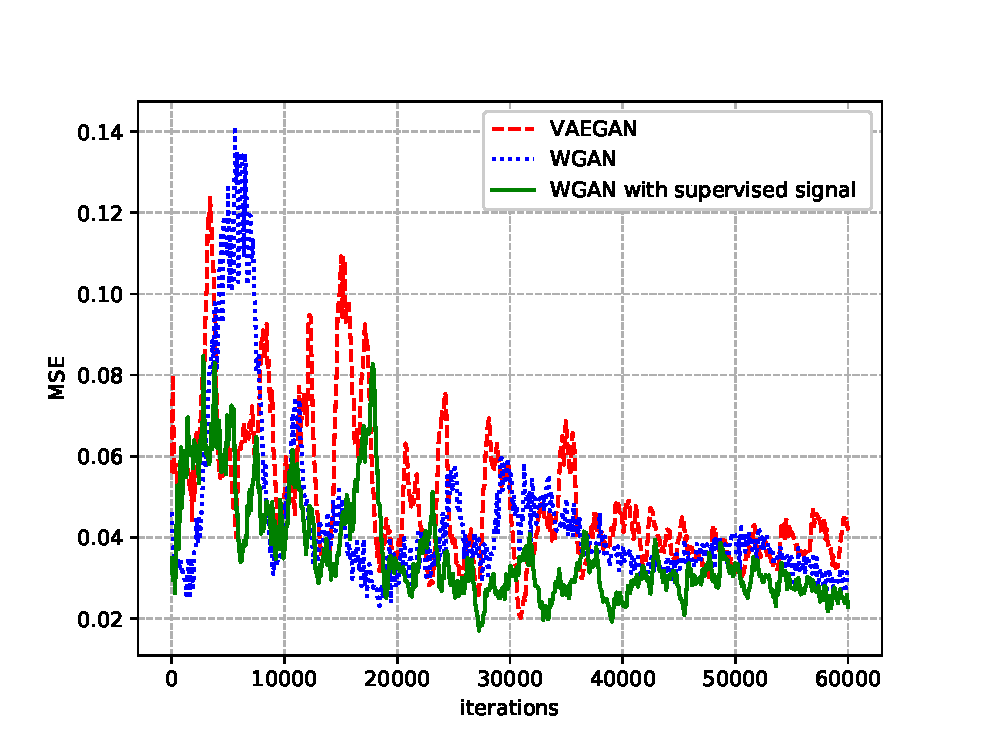
\includegraphics[width=\hsize]{example/3.eps}
	\bicaption[不同模型生成数据进行回归MSE曲线图]
	{不同模型生成数据进行回归MSE曲线图}
	{Mean squared error of different algorithms}
	\label{fig3}
\end{figure}

如图\ref{fig3}所示,改进算法与VAEGAN和WGAN相比收敛速度更快,回归效果更好,反映了改进算法生成的样本更接近原始数据分布。在30000次迭代中,改进算法达到了稳定。由于有监督信号具有固定的先验分布,改进算法在训练初期的MSE明显低于其他算法。

\subsection{对于股票数据的回归}

为了消除实验的偶然性,我们分别对5个股票指数序列数据集进行了算法检验。表\ref{tab1}给出了五种主要的股票价格指数,并使用了代码名。
\begin{table}[htpb]
	\centering
	\bicaption[股票数据详情]
	{股票数据详情}
	{Stock data details.}
	\label{tab1}
	\begin{tabular}{lll} \toprule
		股票价格指数   & 代码名称 &  数据区间  \\  \midrule
		All ordinaries   & AORD&  01/01/2016 to 01/09/2017 \\
		Dow Jones Industrial Average   & DJI&01/01/2016 to 01/09/2017\\
		Hang Seng Index   & HSI&   01/01/2016 to 01/09/2017\\
		KOSPI   & KS11& 01/01/2016 to 01/09/2017\\
		Nikkei Stock Average   &NK&   01/01/2016 to 01/09/2017\\
		\bottomrule
	\end{tabular}
\end{table}
这些数据来自雅虎财经网站\footnote{\url{https://finance.yahoo.com/}}。原始数据包括每天的开盘价、收盘价、最高价、最低价和成交量。这里预测收盘价。采用特征向量法\cite{18},利用最新的价格计算特征来处理序列数据。根据坐标延迟法,输入向量的维数为$m$,延迟时间为$d$,输入向量为$RDP_{1,d},…,RDP_ {m - 1 d}, EMA_{15}$和输出向量$RDP_ {d} $:

\begin{equation}
\label{eq16}
RDP_{i,d} = \frac{p(j)-p(j-i*d)}{p(j-i*d)}*100
\end{equation}


\begin{equation}
\label{eq17}
EMA_{15}  = p(j)-\bar{EMA_{15}(j)}
\end{equation}

\begin{equation}
\label{eq18}
RDP_{d} = \frac{\bar{p(j+d)}-\bar{p(j)}}{\bar{p(j)}}*100
\end{equation}


其中 $p(j)$ 是在时间点 $j$的价格。本文选择延迟时间$d=5$,输入向量维度$m=5$。分割前$80\% $的数据作为训练数据,后$20\% $的数据作为测试数据。分别利用Boostrap,SMOTE,VAEGAN、WGAN和我们算法对转换后的数据进行实验。回归结果如表\ref{tab2}。

\begin{table}[htpb]
	\centering
	\bicaption[股票数据回归结果]
	{股票数据回归结果}
	{Results of stock data regression.}
	\label{tab2}
	\begin{tabular}{lllllll} \toprule		股票名称&随机加权&SMOTE& GAN &  VAEGAN & WGAN &Ours  \\ 
		\midrule
		AORD &0.01356& 0.01023&0.01184 & 0.00667 & 0.00764 &\textbf{0.00622}   \\
		DJI &0.01034&0.00912&0.00816&0.00737&0.00769&\textbf{0.00643}  \\
		HSI &0.01956&0.01834&0.01762&0.01585&0.01612&\textbf{0.01409}  \\
		KS11 &0.02988&0.02765&0.02655&0.02465&0.02621&\textbf{0.02413}\\
		NK  &0.08776&0.06534& 0.07398& 0.03836& 0.04298&\textbf{0.03445} \\
		\bottomrule
	\end{tabular}
\end{table}

如表\ref{tab2}所示,对比于其他模型,改进的算法增强数据在回归问题上获得了更小误差。改进后的算法有两个优点:
\begin{enumerate}
	\item 用自动编码机对数据编码的过程可以获得额外的学习知识,这使得生成器产生的伪样本很难被鉴别器识别。在有监督信号的情况下,生成的数据分布与之前的真实数据分布具有一对一的匹配关系,其对应关系保证生成的网络覆盖了真实数据的所有分布。
	\item 监督信号增强了WGAN输入的先验信息,避免了训练初期由于大量初始化参数而产生的随机样本,加快了训练过程,提升了生成样本的质量。
\end{enumerate}

\section{本章小结}

本章主要介绍了用强化学习模型进行数据增强的生成式对抗网络。在本章的第一部分介绍了数据扩充的意义,GAN的背景,作为生成式模型的一种,GAN相对于传统的其他模型表现出了优良的性能。第二部分介绍了传统数据扩充算法的基本原理以及GAN相关算法的优缺点。在本章的第三部分创新性的提出了引入监督信息的WGAN算法应用于非图像类数据的数据增强,其关键思想是在WGAN与编码器相结合时,通过输入样本的潜在特征来构造真实的样本。在描述改进算法的网络结构和优化的损失函数之后,文中给出了算法具体的实现过程。在文章的第四部分通过可视化的二维数据分析改进算法和其他GAN算法训练曲线和拟合概率密度结果,分析了模型的可行性,在标准数据集下对比传统数据扩充算法证明了改进算法对比传统算法提升效果显著。接着在文章的第五部分,利用新算法分别对实测的电子设备参数数据,和股票数据的回归问题上进行了实验,从理论上和实验上验证了在训练初期,随着对原始参数的大量尝试的减少,改进的引入监督信息的WGAN收敛速度比其他算法都要快,生成的数据更接近真实数据的分布。